%% LaTeX2e class for technical reports
%% techreport.tex
%% 
%% Karlsruhe Institute of Technology
%% Institute for Program Structures and Data Organization
%% Chair for Software Design and Quality (SDQ)
%%
%% Dr.-Ing. Erik Burger
%% burger@kit.edu
%%
%% See https://sdq.kastel.kit.edu/wiki/Dokumentvorlagen
%%
%% Version 1.0, 2023-11-20

%% Available page modes: oneside, twoside
%% Available languages: english, ngerman
%% Available modes: draft, final (see README)
\documentclass[oneside, english]{reports/assets/sdqtechreport}

%% ---------------------------------
%% | Information about the thesis  |
%% ---------------------------------

%% Name of the author
\author{Konstantin Bernhard \and Klim Petraschkevich \and Kristiyan Skordev \and Felix Uhlenbrock \and Justus Zorn}

%% Title (and possibly subtitle) of the thesis
\title{Intrusion Detection using Machine Learning}
\subtitle{Specification}


%% You can put a logo in the ``logos'' directory and include it here
%% instead of the SDQ logo
% \grouplogo{myfile}
%% Alternatively, you can disable the group logo
\nogrouplogo

\date{\today}

\usepackage{graphicx}
\graphicspath{ {./reports/assets} }

%% ====================================
%% ====================================
%% ||                                ||
%% || Beginning of the main document ||
%% ||                                ||
%% ====================================
%% ====================================
\begin{document}

%% Set PDF metadata
\hypersetup{
	pdftitle = {Specification},
	pdfsubject = {Intrusion Detection using Machine Learning},
	pdfauthor = {Konstantin Bernhard, Klim Petraschkevich, Kristiyan Skordev, Felix Uhlenbrock, Justus Zorn}
}

%% Set the title
\maketitle

%% ------------------------
%% |   Table of Contents  |
%% ------------------------
\tableofcontents

%% -----------------
%% |   Main part   |
%% -----------------
\cleardoublepage

%% -------------------
%% | Example content |
%% -------------------

\chapter{Introduction}
\label{chap:Introduction}

In today’s interconnected world, the security of network systems is a critical
concern. As cyber threats continue to evolve, traditional security measures
like firewalls are often inadequate in preventing sophisticated attacks such as
Denial of Service (DoS), flooding, spoofing, and wormhole attacks. These
vulnerabilities can result in system failures, data breaches, and operational
disruptions, emphasizing the need for robust and adaptive security solutions.
This project aims to address these challenges by designing and implementing a
Hybrid Intrusion Detection System (HIDS) that utilizes both rule-based and
anomaly-based detection techniques to identify and mitigate a wide range of
cyber threats in real-time. IDS systems can generally be categorized into two
main types:

\begin{itemize}
	\item Host-Based Intrusion Detection Systems (HIDS): These monitor and analyze
	      activities on individual hosts or devices. They are particularly effective for
	      detecting insider threats, unauthorized file modifications, or privilege
	      escalations. By examining log files, system calls, and other host-specific
	      data, HIDS can provide granular insights into suspicious behavior.
	\item Network-Based Intrusion Detection Systems (NIDS): These focus on monitoring and
	      analyzing network traffic to detect threats like Denial-of-Service (DoS)
	      attacks, packet spoofing, or worms. By capturing and inspecting packets, a NIDS
	      can identify abnormalities and patterns indicative of malicious activities.
\end{itemize}
To enhance detection accuracy, IDS systems employ two primary detection mechanisms:
\begin{itemize}
	\item Anomaly-Based Detection: This approach identifies unusual patterns in system
	      behavior or network traffic that deviate from established baselines. It is
	      particularly effective against novel or previously unknown attacks (zero-day
	      threats), as it does not rely on pre-defined rules. However, it may produce
	      false positives if normal behavior significantly varies.
	\item Signature-Based Detection: This method relies on a database of known attack
	      signatures to identify threats. While highly effective at detecting known
	      vulnerabilities and attacks, it struggles with new or unknown threats for which
	      signatures are unavailable.
\end{itemize}

By analyzing network packets and classifying traffic into normal and malicious
categories, the system enhances the capability to detect unauthorized access
and malicious activities effectively. This comprehensive approach combines
hands-on exploration of network security principles with the power of machine
learning, offering an in-depth learning experience in both fields. Key features
of the HIDS include real-time monitoring, effective alerting mechanisms for
administrators, and logging capabilities for detailed incident analysis.
Optional enhancements, such as developing a user-friendly interface for traffic
visualization and integrating with Security Information and Event Management
(SIEM) systems, expand the system's usability and scope. Furthermore, this
project sets a foundation for future developments, including the adoption of
deep learning models for improved accuracy, encrypted traffic analysis, and
distributed IDS solutions for large-scale networks.

\chapter{Project Scope}
\label{chap:ProjectScope}

As we said we need second defense layer after the firewall. Now we will show in
details against which attacks it is not so robust:

\begin{enumerate}
	\item Denial of service attack – denial-of-service attacks are one of the easiest
	      attacks. They can easily target any system and get useful information from them
	      or make the system fail. This can lead to malfunction of services provided by
	      the system.
	      \begin{enumerate}
		      \item Flooding – It aims to overwhelm a system with superfluous requests, thus
		            preventing legitimate requests from being fulfilled. The primary objective is
		            to make the target service unavailable, either by consuming all its resources
		            or crashing it altogether. Flood attacks exploit the limitations of a network’s
		            bandwidth, memory, and processing power. By sending an excessive number of
		            requests, they can exhaust these resources rapidly, causing severe disruptions.
		            Attackers often use botnets, a network of compromised devices, to generate the
		            enormous volume of traffic required for such attacks, making it harder to trace
		            and block the sources.
	      \end{enumerate}
	\item Confidentiality Threat – Few attackers make programmes which attach themselves
	      to the existing files, they corrupt them or make a copy which can be leaked or
	      distributed via email. This leads to confidentiality threat for the author as
	      this action is being taken without his permission.
	\item Modify the contents – Intruders can change the content or they can even make
	      hoax broadcasts from authors system all this can have an economic impact. \item
	      \begin{enumerate}
		      \item Masquerade – An attack that involves the use of a manipulated, spoofed or
		            stolen user identifier – device, digital signature, network address,
		            certificate, etc. – to fool digital infrastructure and gain access to systems,
		            or authorization to conduct certain privileged actions. Masquerade attacks can
		            be used to perpetuate financial crime, compromise corporate systems, or access
		            sensitive data.
		      \item Spoofing – When someone is sitting in between the communication, capturing the
		            packets and deliver changed ones. Both communication partners do not know about
		            him. They think, they are communicating directly with each other, but they
		            don't. Also, the packets information could be changed without notice. So, this
		            could be used for hacking.
	      \end{enumerate}
	\item Wormhole – This is a type of network layer attack which is carried out using
	      more than one malicious node. The nodes used to carry out this attack are
	      superior to normal nodes and are able to establish better communication
	      channels over long ranges. The idea behind this attack is to forward the data
	      from one compromised node to another malicious node at the other end of the
	      network through a tunnel. As a result, the other nodes in the WSN can be
	      tricked into believing that they are closer to other nodes than they really are
	      which can cause problems in the routing algorithm.
\end{enumerate}

It is important to note that our system does not contain prevention. The only
thing it can do in case of attack detection is to inform the customer or the
administrator and for instance isn’t fit to block the IP of the intruder or the
offending data. Also, it is not capable to check encrypted traffic. The IDSs
are placed at such points so that all the packets, devices, files and the
traffic could be checked. That could be individual hosts or devices. On servers
that provide communication with foreign systems, is desirable to be installed
anti-threat software and firewall, antivirus software and spyware-detection –
on all of the networks.

\chapter{Implementation}
\label{chap:Implementation}

\section{Project Overview}
\label{sec:ProjectOverview}

Our project is structured into three key phases (modules) to build an efficient
Hybrid Intrusion Detection System (HIDS). Each phase serves a distinct purpose,
combining to ensure comprehensive protection against malicious network
activity. These modules are:

\begin{enumerate}
	\item Module 1: Packet Capture – Captures all incoming network packets to the host
	      system.
	\item Module 2: Rule-Based Detection – Applies predefined rule-based filters to
	      identify known malicious patterns.
	\item Module 3: Anomaly-Based Detection – Uses machine learning techniques to detect
	      anomalous or previously unseen patterns.
\end{enumerate}

This layered approach allows us to effectively detect both known and unknown
threats.

\section{Module 1: Packet Capture}
\label{sec:PacketCapture}

Purpose: The Packet Capture module is responsible for capturing live network
traffic arriving at the host system. This raw traffic data is then processed
and forwarded to the subsequent modules (Rule-Based and Anomaly-Based
Detection) for detailed analysis. This module ensures that all relevant data
points, such as IP addresses, ports, and protocol details, are extracted and
structured.

Core Functionality:
\begin{enumerate}
	\item Packet Sniffing:
	      \begin{itemize}
		      \item The module monitors the network interface to capture incoming packets in
		            real-time.
		      \item Captured packets include essential metadata such as source/destination IP, MAC
		            addresses, protocols (TCP, UDP, ICMP), and port numbers.
	      \end{itemize}
	\item Packet Processing:
	      \begin{itemize}
		      \item Extracts key details (e.g., headers, protocol flags, payloads) from captured
		            packets.
		      \item Converts this data into a structured format to ensure compatibility with
		            downstream modules.
		      \item Filtering and Optimization:
	      \end{itemize}
	      \begin{itemize}
		      \item Initial filtering is applied (e.g., capturing only TCP/UDP traffic).
		      \item Packets are logged for further analysis or debugging.
	      \end{itemize}
\end{enumerate}
\section{Technology used: Scapy Library}
\label{sec:ScapyLibrary}

To implement the Packet Capture module, we use the Scapy library in Python,
which is a powerful tool for packet sniffing and network analysis. Why Scapy?

\begin{itemize}
	\item Flexibility: Scapy provides robust methods for capturing, processing, and
	      analyzing network packets across various protocols (e.g., IP, TCP, UDP).
	\item Ease of Use: It is beginner-friendly and allows us to build packet sniffers and
	      analyzers with minimal code complexity.
	\item Extensibility: Scapy supports both real-time packet sniffing (using the sniff
	      function) and detailed protocol dissection (e.g., IP, TCP headers).
	\item Customizability: Packets can be filtered and manipulated according to project
	      requirements, which simplifies the implementation of rule-based and
	      anomaly-based filters.
\end{itemize}

How Scapy Works:

\begin{enumerate}
	\item Packet Capture: Scapy's sniff() function is used to monitor and capture packets
	      on a specified network interface. Example: Capturing only TCP packets:
	      sniff(filter="tcp", prn=packet\_handler)
	\item Packet Dissection: Captured packets are dissected into layers (e.g., Ethernet,
	      IP, TCP), allowing access to individual attributes like src, dst, flags, etc.
	\item Integration: Once processed, the captured packet data is forwarded to Modules 2
	      and 3 for further analysis.
\end{enumerate}

Output of Module 1: The output of this module will be a structured
representation of captured packets, containing:

\begin{itemize}
	\item Source and Destination IPs
	\item MAC Addresses
	\item Protocol Types (e.g., TCP, UDP, ICMP)
	\item Port Numbers
	\item Payload or Flags
\end{itemize}

This data will be stored or directly sent to Modules 2 and 3 for:

\begin{itemize}
	\item Rule-Based Detection: Matching against predefined signatures.
	\item Anomaly-Based Detection: Feeding into machine learning algorithms.
\end{itemize}
\section{Module 2: Rule-Based Detection}
\label{sec:RuleBasedDetection}

This module focuses on identifying malicious packets using predefined rules and
signatures. It serves as the first layer of protection by filtering out known
threats based on established criteria.

Core Functionality:
\begin{enumerate}
	\item Signature Matching: Compares packet attributes (e.g., IP headers, TCP flags,
	      ports) against a database of known malicious patterns. Example rules include
	      detecting:
	      \begin{itemize}
		      \item Illegal TCP flag combinations (e.g., SYN-FIN).
		      \item Broadcast destination addresses (e.g., .255).
		      \item Reserved or suspicious IP addresses.
	      \end{itemize}
	\item Actions: If a match is found, the packet is flagged as malicious, and an alert
	      is generated.
\end{enumerate}

Advantages:

\begin{itemize}
	\item High Efficiency: Quickly identifies known attacks with minimal computation.
	\item Deterministic: Provides reliable detection for documented attack patterns.
\end{itemize}
\section{Module 3: Anomaly-Based Detection}
\label{sec:AnomalyBasedDetection}

This module utilizes machine learning techniques to identify unusual or
suspicious activity that deviates from normal network behavior. It acts as the
second layer of protection to detect previously unseen or evolving threats.

Core Functionality:
\begin{enumerate}
	\item Baseline Analysis: Models normal network behavior using training data (e.g.,
	      NSL-KDD dataset).
	\item Real-Time Classification:
	      \begin{itemize}
		      \item Analyzes live traffic using a trained model (e.g., Support Vector Machine).
		      \item Flags packets that exceed predefined thresholds as potential anomalies.
	      \end{itemize}
	\item Self-Improvement: Continuously refines the model with new data to adapt to
	      changing attack patterns.
\end{enumerate}

Advantages:
\begin{itemize}
	\item Dynamic and Adaptive: Capable of detecting zero-day attacks and novel threats.
	\item Complements Rule-Based Detection: Bridges the gap left by static
	      signature-based methods.
\end{itemize}

\chapter{Alerts}
\label{chap:Alerts}

Alerts are used to notify the administrator of suspicious activity, even while
the administrator is not actively checking the IDS or even working at all.

\section{Alert Content}
\label{sec:AlertContent}

Since the administrator might not be working when they receive an alert, the
alert MUST include all information necessary for the administrator to take
action, including:

\begin{itemize}
	\item The exact time and date of the attack, so that the administrator knows whether
	      it is still in progress or already over.
	\item The type and severity of the attack, since certain attacks (e.g. DoS) only
	      cause downtime, while others (e.g. SQL injection) can cause data leakage and
	      are therefore much more problematic.
	\item How certain the IDS is that this is an actual attack, instead of normal
	      behavior. This is especially important since an administrator may take actions
	      in response to threats that are themselves a threat to the network, e.g.
	      shutting down servers immediately (which might cause data loss and downtime).
	      If the IDS provides a certainty score (between 0 and 1), the administrator
	      knows whether they should inspect the attack more closely first or take action
	      immediately.
	\item A hyperlink to a webpage (in the user interface, if developed) that contains
	      further information about the exact notification the administrator received.
\end{itemize}

\section{Alert Delivery}
\label{sec:AlertDelivery}

It is likely that most attacks happen while the administrator is not paying
close attention to the system, so it is essential that the alerts are delivered
within a couple of seconds and that they are loud enough to alarm the
administrator, potentially even during the night. Otherwise, the attack might
be over before the administrator even notices that anything happens.

The obvious choice for alert delivery is a messenger, which is typically
installed on mobile devices. Since messengers are used for asynchronous
communication between people, they often include functionality to notify the
user, even while not looking at the device. Typical ways of achieving this are
a notification sound or vibration.

Many messengers, especially those built for communication in bigger teams,
include functionality to send messages automatically, i.e. from other services.
This is achieved using webhooks, which means that the messenger service is
listening on the network, and our IDS can send a request via the HTTP protocol,
which will then send a message to the intended user. Common examples of
messengers implementing such functionality are Mattermost, Slack, and Teams.

To make our IDS more flexible and not fix it to a certain messenger service, it
MUST have the ability to send webhook requests to arbitrary servers, which can
be configured by the administrator. These webhook requests MUST be in the JSON
data format, and sent via the HTTP POST protocol to a user-provided URL. The
structure of the requests is as follows:

\begin{verbatim}
{
	"timestamp": <UNIX time stamp>,
	"attack": <name of attack>,
	"severity": <one of low, medium, high>,
	"certainty": <score between 0 and 1, 0: uncertain, 1: certain>,
	"link": <link to a webpage with further details, if implemented>
}
\end{verbatim}

The exact names of the attacks as well as the assigned severities and
certainties depend on the database used for the IDS. The administrator can
write a service themselves which provides a webhook and configure the IDS to
send all alerts to this webhook. This service will then be responsible for
parsing the above datastructure, and sending webhooks to the actual messenger
services. While this is more effort for the administrator, it makes the IDS
completely independent of the messenger service used for delivering the alerts
to the user. If possible, the project SHOULD contain at least one example for
such a service which delivers alerts to an actual messenger service.

\begin{center}
	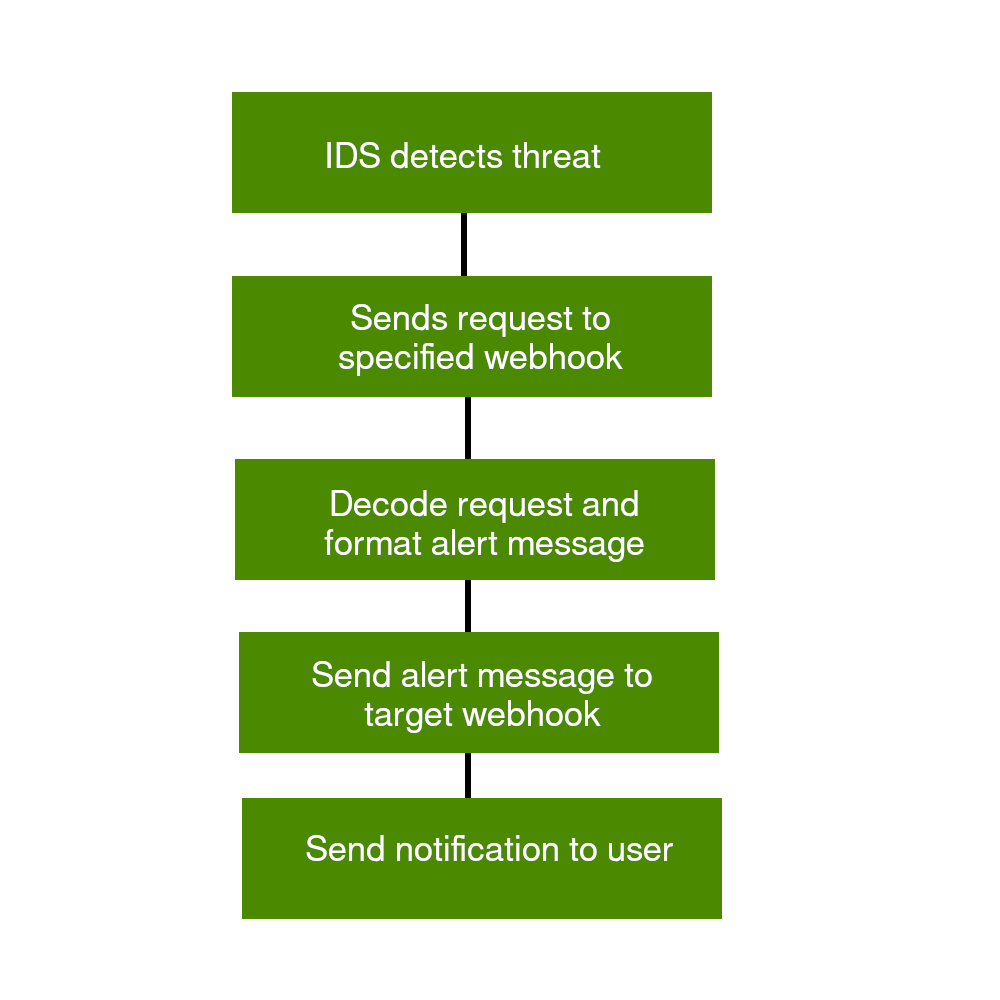
\includegraphics{alert-workflow}
\end{center}

\chapter{User Interface}
\label{chap:UserInterface}

While not essential to our project, the IDS SHOULD contain a user interface
that provides the administrator with deeper insights into their network. The
user interface SHOULD be provided as a simple website, served directly from the
main deployment, i.e. there MUST be no separate website server.

The UI SHOULD consists of three different parts:
\begin{itemize}
	\item An overview of the system
	\item Detail pages for the individual alerts
	\item Configuration options for the IDS
\end{itemize}

\section{Overview}
\label{sec:UserInterfaceOverview}

The overview MUST contain some statistics to assess health, including but not
limited to:

\begin{itemize}
	\item The total number of packets processed, so the administrator can easily assess
	      whether the system is overloaded.
	\item The average duration packet processing takes, so the administrator can detect
	      when the IDS itself is overloaded.
	\item The amount of alerts sent, and how many of these were marked as correct by the
	      administrator. This can help the administrator to adjust settings related to
	      the false-positive rate of the IDS.
\end{itemize}

Also, the overview MUST contain a list of currently active alerts, which is all
alerts that were triggered but not yet reviewed by the administrator. This list
MUST contain exactly the information that is also present in the alert HTTP
requests, as specified in section \ref{sec:AlertDelivery}. Clicking on a single
alert leads to the alert display page specified in section
\ref{sec:UserInterfaceAlertDetails}.

\section{Alert Details}
\label{sec:UserInterfaceAlertDetails}

The alert details MUST contain the information already provided in the alert
itself, i.e.

\begin{itemize}
	\item Timestamp
	\item Attack type
	\item Attack severity
	\item Certainty
\end{itemize}

It MAY also contain further descriptions:

\begin{itemize}
	\item An overview of the attack, in case the administrator is not familiar with it.
	      This description MAY be sourced from a database, or generated by the system
	      automatically.
	\item An estimate of the effect the attack would have, which explains the severity.
	      This may e.g. include whether the IDS estimates the attack would succeed, or
	      which services could be affected.
	\item A proposed plan of action. This MAY also be sourced from a database, or
	      generated by the IDS. In any case, the IDS should never perform such actions
	      automatically, and the administrator should only view this plan of action as a
	      hint, and not rely on it.
\end{itemize}

The alert details page MUST include buttons for reviewing the attack:

\begin{itemize}
	\item Dismiss: When the administrator clicks this button, the alert is removed from
	      the active alert list on the overview page. This information SHOULD be used to
	      train the IDS or adjust the settings, so that the number of false positives may
	      be reduced.
	\item Resolved: When the administrator clicks this button, the alert is also removed
	      from the active alert list. This information MAY also be used to further train
	      the IDS.
\end{itemize}

The page MAY include a text field for notes the administrator can use to
associate information with this specific type of attack, or the alert itself.

\section{Settings}
\label{sec:UserInterfaceSettings}

The settings page allows the administrator to configure how the IDS works:

\begin{itemize}
	\item It MUST provide a way to configure the webhook URL, which determines where
	      alerts are sent. This is specified in section \ref{sec:AlertDelivery}.
	\item It SHOULD provide a minimum certainty level, which allows the administrator to
	      adjust how certain the IDS has to be before sending an alert. This is important
	      to adjust the false-positive rate to an acceptable level.
	\item It SHOULD provide options specific to the exact model used by the IDS.
	\item It MAY provide a list of previously reviewed alerts, and the option to change
	      the review of these (in case the review was wrong).
	\item It MAY provide a way to add signatures or similar to influence the
	      decision-making process of the IDS directly.
\end{itemize}

\section{Preliminary Designs}
\label{sec:UserInterfaceDesigns}

Overview page:

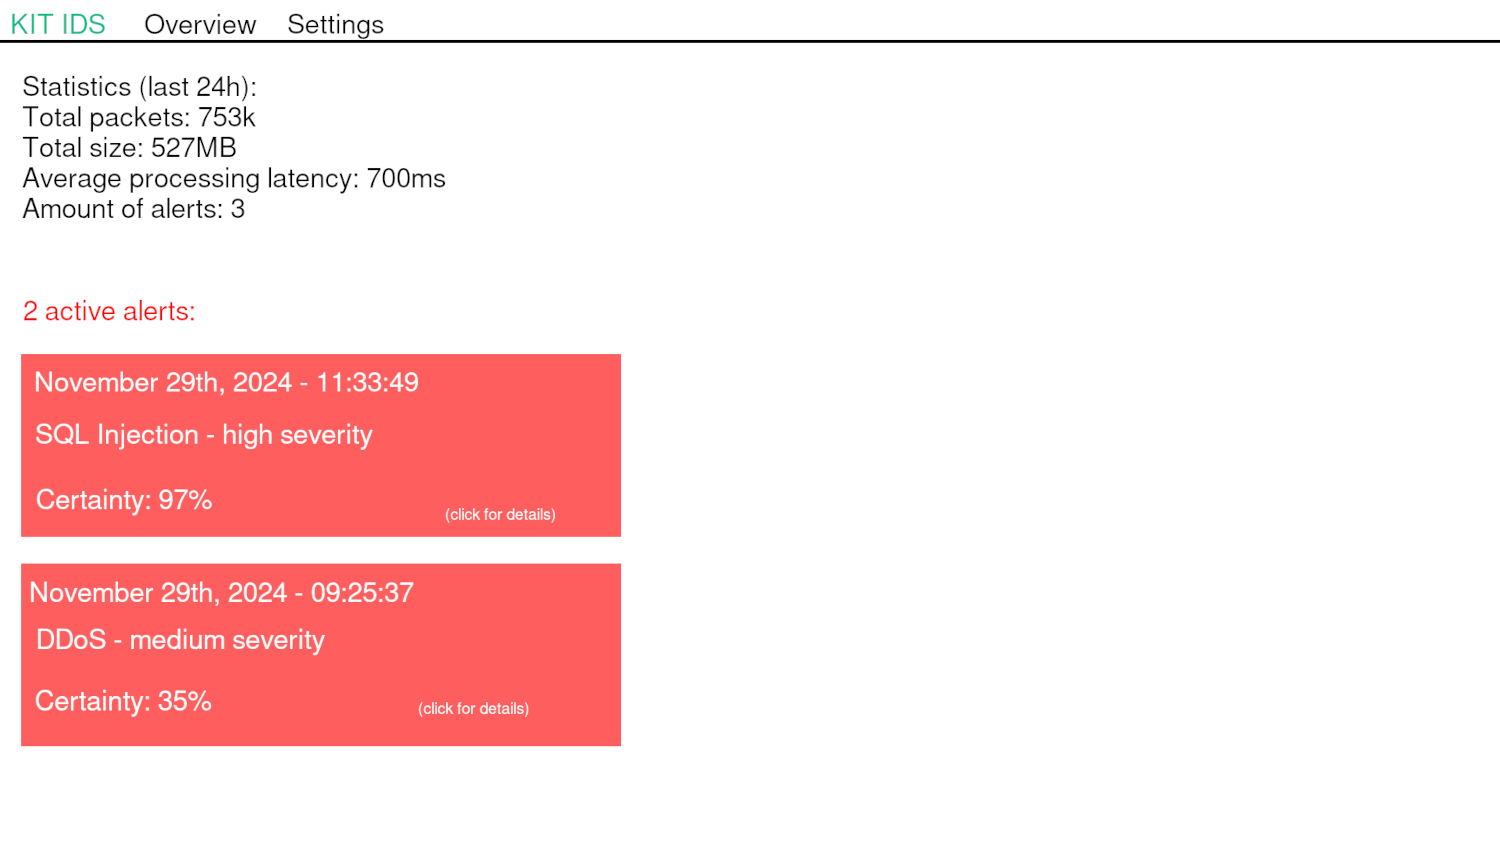
\includegraphics{ui-overview}

Alert details page:

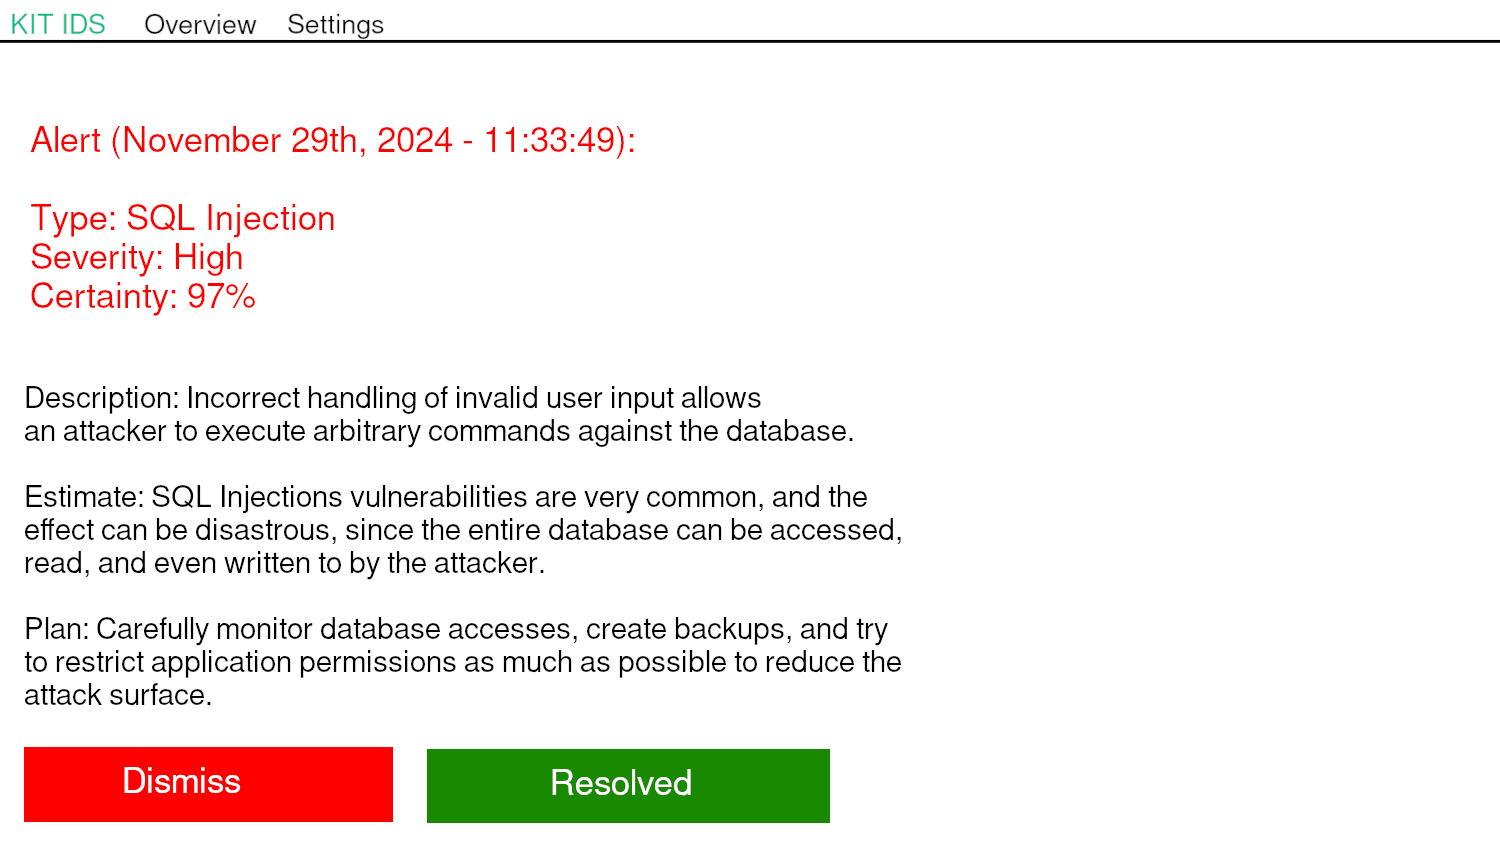
\includegraphics{ui-details}

Settings page:

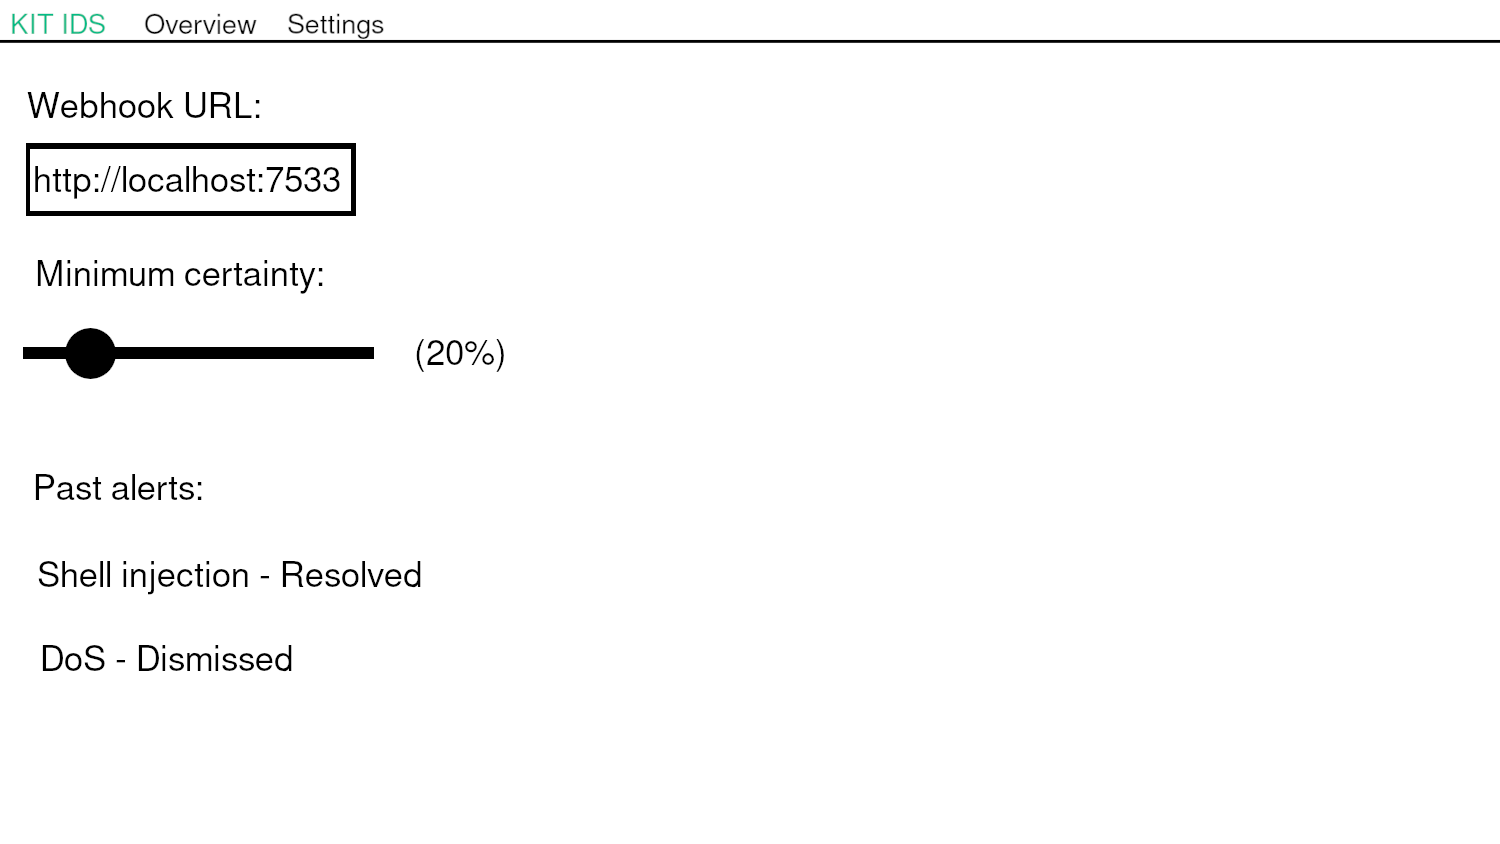
\includegraphics{ui-settings}

\chapter{Use Cases}
\label{chap:UseCases}

Mandatory:

\begin{enumerate}
	\item Start and Stop IDS: \\Actors: User. \\Description: The user should be able to start
	      and stop the capturing and detection of malicious packets. \\Precondition: IDS is
	      installed. \\Normal procedure: User starts the process through a command or
	      click. IDS starts monitoring the traffic. User can stop the IDS from monitoring
	      through a command or click. \\Alternative procedure: If the IDS was not installed
	      properly or the database is corrupt, the IDS should display an error message.
	      \\Result: The administrator can control the IDS system to start or stop
	      monitoring.
\end{enumerate}

Optional:

\begin{enumerate}
	\item Model Performance Display: \\Actors: User. \\Description: The GUI enables users to
	      view the performance metrics of the machine learning model used by the IDS.
	      \\Precondition: IDS is installed. \\Normal procedure: User navigates to the details
	      of the machine learning model in the GUI. The system displays the performance.
	      The system updates the performance while the IDS is running. \\Alternative
	      procedure: If the model was not loaded or no data is available, the GUI should
	      display a message informing the user about the problem. \\Result: The user can
	      get information on the effectiveness and reliability of the model.
	\item Notification Log: \\Actors: User. \\Description: The GUI enables users to view the
	      log of all the notifications and the details about the identified packages.
	      \\Precondition: IDS is installed. \\Normal procedure: User navigates to the details
	      of the log in the GUI. The system displays the log. The log can be filtered,
	      sorted by attributes. The system updates the log while the IDS is running.
	      \\Alternative procedure: If there is no log, a message like “No log available”
	      should be displayed. \\Result: The user can get information on the detected
	      packages.
\end{enumerate}

\chapter{Test Cases}
\label{chap:TestCases}

Mandatory:

\begin{enumerate}
	\item Packet Capture: \\State: IDS running, network is active. \\Action: Start packet
	      capturing \\Expected reaction: IDS captures packets from the network.
	\item Corrupt Database: \\State: The Database is corrupted, for example some signature
	      being invalid. \\Action: User tries to start the IDS. \\Expected Reaction: IDS
	      displays an error message.
	\item Signature-Based Intrusion Detection: \\State: Database contains known malicious
	      signatures. \\Action: A packet with a known malicious signature is being send.
	      \\Expected reaction: IDS notifies the user and logs the alarm.
	\item Machine-Learning-Based Detection: \\State: IDS is running, using the Model that
	      has been trained with a dataset. \\Action: A malicious packet was send and has
	      bypassed the first layer. \\Expected reaction: IDS notifies the user and logs the
	      alarm and adds the new signature to the database.
	\item False Positive: \\State: IDS is running, using the Model that has been trained
	      with a dataset. \\Action: A safe Packet is being send. \\Expected reaction: IDS
	      does not notify the user.
\end{enumerate}

Optional:

\begin{enumerate}
	\item GUI working: \\State: IDS is running. \\Action: User opens GUI through a command or
	      click. \\Expected reaction: Interface appears with information on the current
	      traffic.
	\item Change in the Database: \\State: Database contains known malicious signatures.
	      \\Action: The User adds or deletes a new Signature through the interface.
	      \\Expected reaction: The database is updated correctly and the IDS is able to use
	      the new signature in future packet analysis.
\end{enumerate}

\end{document}
